\documentclass[crop,class=article]{standalone}
%----------------------------Preamble-------------------------------%
\usepackage{tikz}                       % Drawing/graphing tools.
\usetikzlibrary{
    calc,                   % Calculating right angles and more.
    arrows.meta,            % Latex and Stealth arrows.
    decorations.markings,   % Adding arrows in the middle of a line.
}
%--------------------------Main Document----------------------------%
\begin{document}
    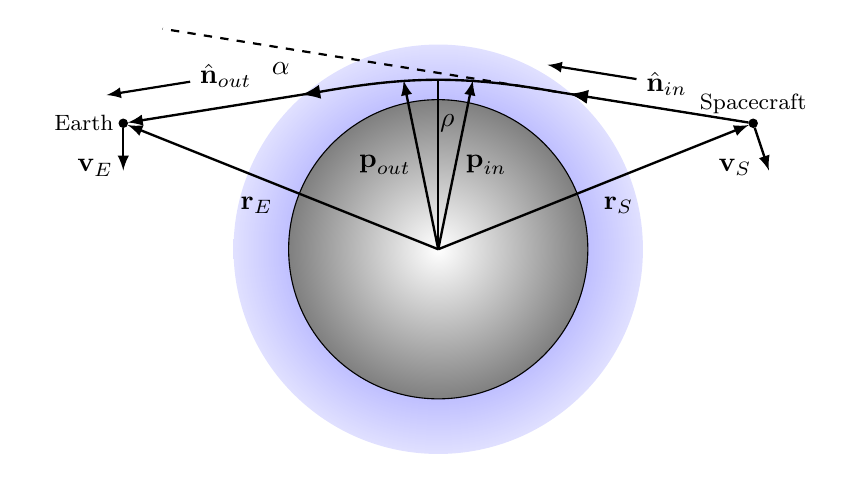
\begin{tikzpicture}[>={latex[black]}]
        \begin{scope}[
            every node/.style={
                circle,
                fill=black,
                draw=black,
                inner sep=0pt,
                minimum size=3pt
            }
        ]
            \node (S) at (4,1.6) {};
            \node (E) at (-4,1.6) {};
        \end{scope}
        \coordinate (O) at (0,0);
        \coordinate (p1) at (-1.5,2);
        \coordinate (p2) at (1.5,2);
        \coordinate (P) at (0,2.2);
        \coordinate (dash) at (-3.5,2.8);
        \node at (E) [left] {\footnotesize{Earth}};
        \node at (S) [above] {\footnotesize{Spacecraft}};
        \draw[%
            draw=none,
            inner color=blue,
            outer color=white!80!blue,
            opacity=0.6
        ]   (0,0) circle (26mm) (0,0) circle (1.9);
        \draw[inner color=white, outer color=gray]
            (0, 0) circle (1.9);
        \begin{scope}[line width=0.3mm,->]
            \draw[%
                postaction={decorate},
                decoration={%
                    markings,
                    mark=at position .29 with \arrow{Latex},
                    mark=at position .72 with \arrow{Latex}
                }
            ]   (S) to (p2)
                    to[bend right=10] (p1)
                    to (E);
            \path (O) edge node[right] {$\textbf{p}_{in}$} (0.44,2.144);
            \path (O) edge node[left] {$\textbf{p}_{out}$} (-0.44,2.144);
            \path (O) edge node[below left] {$\mathbf{r}_{E}$} (E);
            \path (O) edge node[below right] {$\mathbf{r}_{S}$} (S);
            \path (S) edge node[below left] {$\mathbf{v}_{S}$} (4.2,1);
            \path (E) edge node[below left] {$\mathbf{v}_{E}$} (-4,1);
        \end{scope}
        \node (nin) at (2.9,2.1) {$\hat{\mathbf{n}}_{in}$};
        \node (nout) at (-2.7,2.2) {$\hat{\mathbf{n}}_{out}$};
        \draw[thick] (O) to (0,2.15);
        \draw[thick,shorten >=1cm,shorten <=0cm,->]
            (nin) -- +($(p2)-(S)$);
        \draw[thick,shorten >=1cm,shorten <=0cm,->]
            (nout) -- +($(E)-(p1)$);
        \draw[thick,dashed] (p2) -- (dash);
        \node at (-2,2.3) {$\alpha$};
        \node at (-0.1,1.6) [right] {$\rho$};
    \end{tikzpicture}
\end{document}